%% LaTeX Beamer presentation template (requires beamer package)
%% see http://latex-beamer.sourceforge.net/
%% idea contributed by H. Turgut Uyar
%% template based on a template by Till Tantau
%% this template is still evolving - it might differ in future releases!

% Voyager presentation for Developers Workshop 2007
% Adrian Gschwend

\documentclass{beamer}
% Handout:
%\documentclass[handout]{beamer}

\mode<presentation>
{
\usetheme{Warsaw}
\setbeamercovered{transparent}
}

\usepackage{amsmath,amssymb}
\usepackage[latin1]{inputenc}
\usepackage{times}
\usepackage[T1]{fontenc}

\beamertemplatetransparentcovereddynamic

%\logo{
\includegraphics[height=0.5cm]{dws06.png}}

\title[netlabs.org - The Voyager Project]
{netlabs.org - The Voyager Project}

\subtitle
{Where Are We Now?}

\author[Adrian Gschwend]
{Adrian~Gschwend}

\institute[netlabs.org]
{
netlabs.org - Open Source Software
}

\date[07.07.2007]
{Developers Workshop 2007, Amsterdam, Netherlands}

\subject{OS/2 and eCS development}
\keywords{OS/2 eCS eComStation Voyager}

% \AtBeginSubsection[]
% {
% \begin{frame}<beamer>
% \frametitle{Overview}
% \tableofcontents[part-1]
% \end{frame}
% }


\begin{document}

\begin{frame}
\titlepage
\end{frame}

\begin{frame}
\frametitle{Outline}
\tableofcontents[hideallsubsections]
\end{frame}

\section{History}

\subsection{The Journey}
\begin{frame}[allowframebreaks=0.6]
\frametitle{The Idea}
The Story so Far\ldots
\begin{itemize}
  \item Long process of thinking about the future for several years
  \item First idea with Kernel of MacOS X in Summer 2004
  \item First presentation of that idea at Developers Workshop 2005 in Dresden
  \item Reconsideration of this idea because it doesn't solve the main problem: Desktop
  \item New idea with OpenGL based Desktop with well known toolkits, developed at SYSTEMS fair in Munich
  \item Talks to various people and first presentation of that idea at
  Warpstock Europe 2005 in Dresden
  \item Presentation of first concept and design studies at Developers
  Workshop 2006 in Biel, Switzerland
  \item License decision during Summer 2006
  \item First 0.1 release of \textit{The Design of Voyager} released to the
  public for Warpstock Canada 2006
  \item Coding from various site, namely Chris Wohlgemuth on NOM
  \item Design studies for GTK+ on OS/2 by Dmitry
  \item Happy Hacking in Wintercamp 2007
  \item No more progress on the DOV document because Adrian was in long holidays\ldots
  \item but, progress on the projects itself, thanks to everyone!
\end{itemize}
\end{frame}

\begin{frame}
\frametitle{Voyager (R)evolution}
\begin{itemize}[<+->]
  \item Development of Voyager should be possible on many platforms, starting on
  eCS
  \item Support for the most popular Unix-like systems is required
  \item Support for Windows is a must
  \item eCS developers should be motivated to use SOM for new ideas because
  code can be partially reused
  \item Users can continue to use eCS as we know it today and still get new features
  \item Part-by-part replacement for smooth migration
\end{itemize}
\end{frame}

\begin{frame}
\frametitle{The Vision}
There is more to do\ldots
\begin{itemize}[<+->]
  \item A team of interested developers might start working on an OS/2 compatibility layer for Unix-like systems
  \item In long term we need a new kernel (discussion is open, see kernel
  presentation at DWS 07)
  \item Most of the OS/2 coders don't like the Linux design so other options are preferred
  \item Final goal: our own distribution based on existing and new software
\end{itemize}
\end{frame}

\section{The Voyager Project}
\subsection{Introduction}

\subsection{Design of Voyager}
\begin{frame}
\frametitle{Voyager Components, now}
\begin{itemize}[<+->]
  \item Netlabs Object Model (SOM)
  \item Voyager Desktop (WPS)
  \item Cairo (GPI/GDI)
  \item GTK+ (GUI Toolkit, PM)
  \item Triton (Multimedia Subsystem, MMPM/MMOS2)
\end{itemize}
\end{frame}

\begin{frame}
\frametitle{Voyager Components, next steps}
\begin{itemize}[<+->]
  \item Proper security concept
  \item Neptune (Window Manager for Cairo and Xlib)
  \item OpenGL based Cairo backend
  \item Xorg OpenGL device drivers (no Xlib necessary in mid-term)
\end{itemize}
\end{frame}

\section{Voyager Components}
\subsection{Under Development}

\begin{frame}
\frametitle{Netlabs Object Model}
\begin{itemize}[<+->]
  \item SOM is a binary compatible object model, no need to recompile objects (unlike on GNOME for example)
  \item There are some design documents from IBM itself (published in ACM)
  \item There is quite some documentation available written by former IBM employees
  \item Chris Wohlgemuth started to re-implement the concepts under the name NOM
  \item This is the base for a WPS like desktop
\end{itemize}
\end{frame}

\begin{frame}
\frametitle{NOM Design}
%\begin{columns}
%\column[T]{5cm}
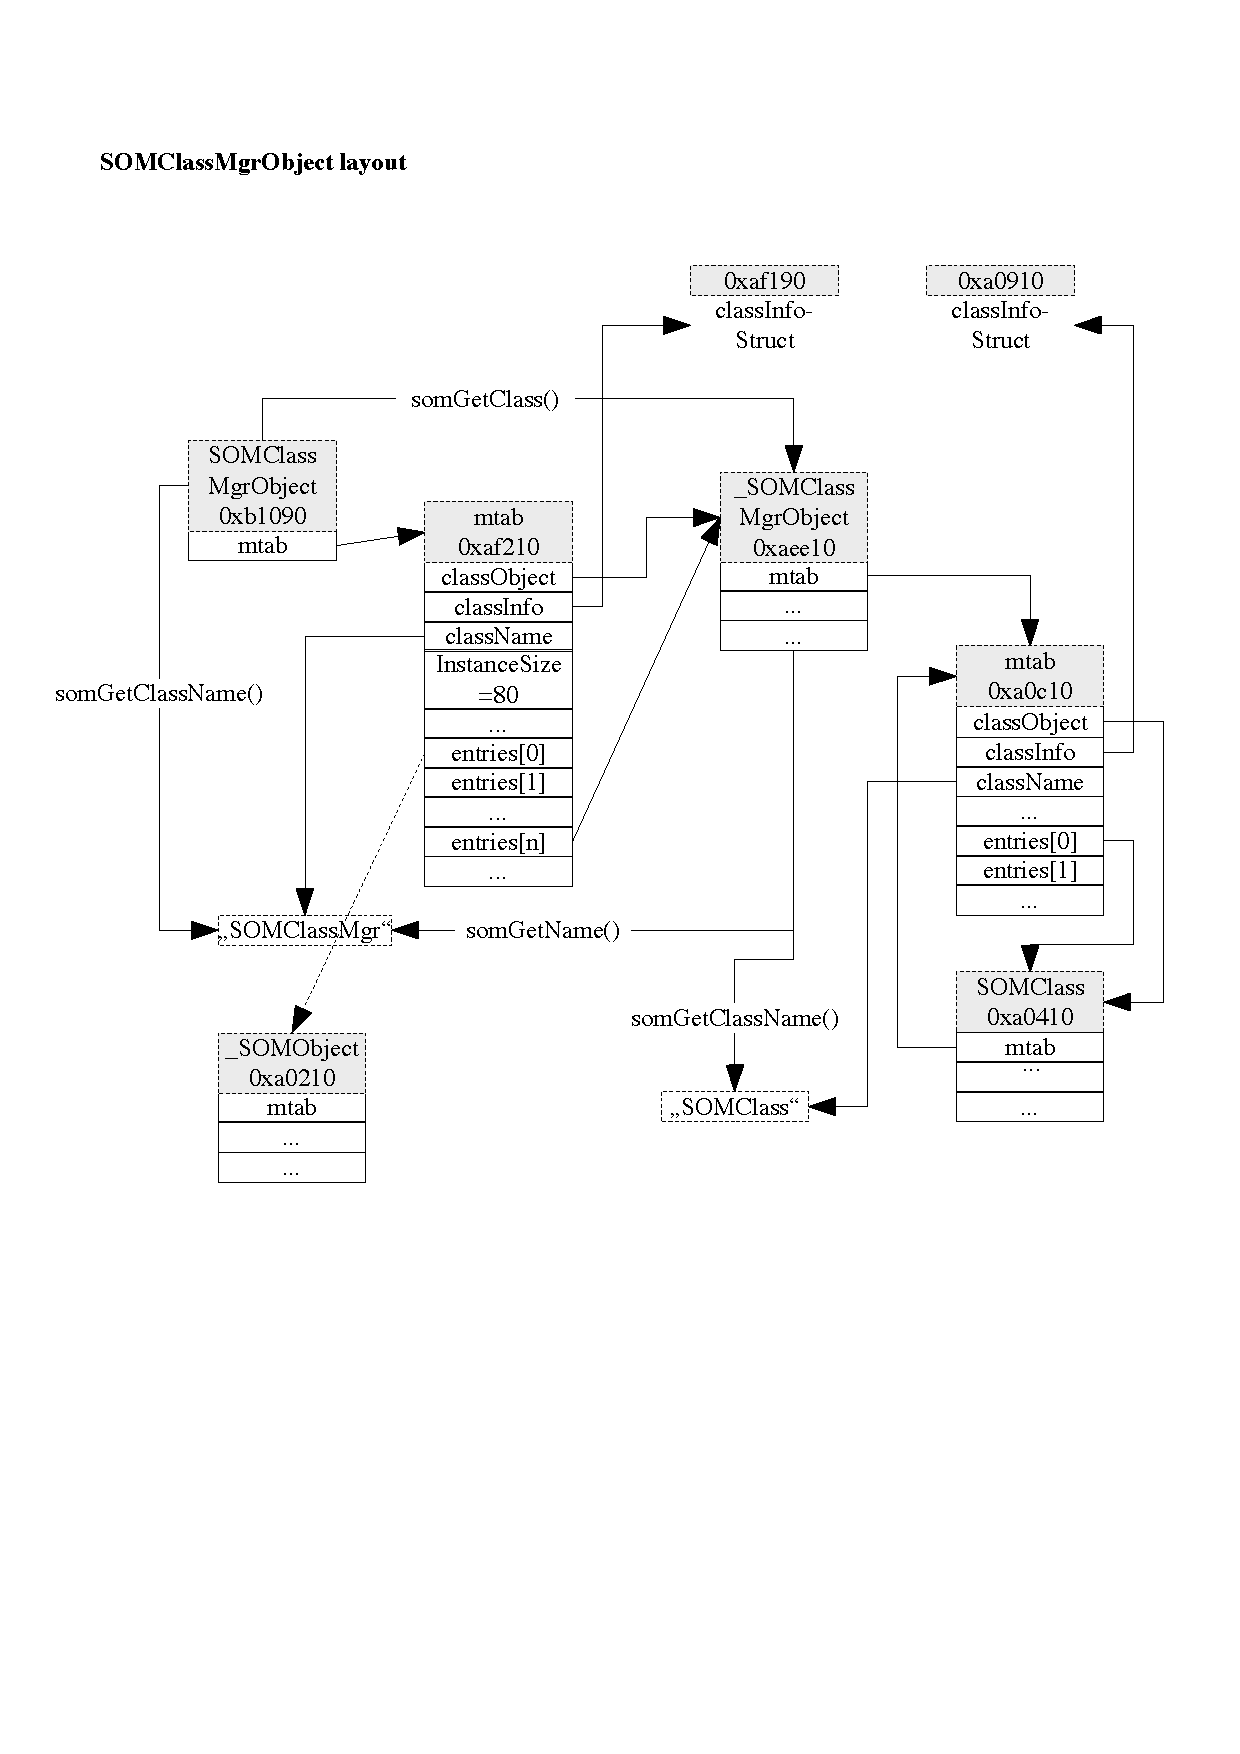
\includegraphics[width=8cm]{images/SOMClassMgrObject-layout.pdf}
%\column{5cm}
%Simplified design of the Xorg OpenGL backend (taken from official docs), Xlib stripped out
%\end{columns}

\end{frame}

\begin{frame}
\frametitle{Netlabs Object Model}
Things that work right now:
\begin{itemize}[<+->]
  \item Binding files creation (IDL compiler)
  \item Class creation from IDL files
  \item Subclassing
  \item Method overriding
\end{itemize}
\end{frame}

\begin{frame}
\frametitle{Netlabs Object Model}
Thinks that do not work yet:
\begin{itemize}[<+->]
  \item Class replacement, almost done
  \item Dynamical loading of classes, in development
  \item \ldots
\end{itemize}
Difference to SOM:
\begin{itemize}[<+->]
  \item Use of an environment pointer in each method call (CORBA exception
  handling)
  \item SOM specific IDL extensions are not supported
  \item No distributed SOM
  \item Object pointer check
  \item \ldots
\end{itemize}
\end{frame}

\begin{frame}
\frametitle{Voyager Desktop}
\begin{itemize}[<+->]
  \item WPS classes in development now
  \item Subversion available, code checked in
  \item Roadmap needed, discussion open! Target: 1.0 release
\end{itemize}
Summary: There is quite a lot of code available for Voyager - no vaporware :-)
\end{frame}

\begin{frame}
\frametitle{Cairo}
\begin{itemize}[<+->]
  \item modern, open source, cross-platform 2D API
  \item PDF/PS-like 2D API (hint: MacOS X Quartz)
  \item multiple output systems (screen, printer)
  \item OS/2 port exists, not accelerated so far
  \item OpenGL based backend exists, called Glitz (hint: MacOS X Quartz :)
\end{itemize}
\end{frame}

\begin{frame}
\frametitle{GTK+ Toolkit}
\begin{itemize}[<+->]
  \item Most used toolkit on Unix-like systems nowadays
  \item LGPL license (binary linking possible, unlike qt)
  \item Abstraction layer called GLIB
  \item Ongoing development (well, somewhat)
  \item wxWidgets and SWT are implemented on top of it
  \item Not yet available on eCS, PM port is evaluated right now
  \item We might need to enhance it in mid-term
\end{itemize}
\end{frame}

\begin{frame}
\frametitle{Triton}
\begin{itemize}[<+->]
	\item Well-defined subsystem
	\item Core library
	\item Easy-to-use API for the application developers to visualize and control multimedia contents
	\item Easy-to-use API for the plugin developers to be able to extend the system with support of new multimedia formats
\end{itemize}
\end{frame}

\begin{frame}
\frametitle{Triton Status}
\begin{itemize}[<+->]
  \item First audio codec implemented: MP3 (April 2006)
  \item First image codecs implemented: GBM module support
  \item First video codec implemented: (can't remember which one ;)
\end{itemize}
\end{frame}

\subsection{Next Steps}

\subsection{OS/2 and eCS Compatibility}
\begin{frame}
\frametitle{Some Ideas}
People do ask for binary compatibility. We see the following options:
\begin{itemize}[<+->]
  \item Use a pure VM based solution - easy and will work well
  \item Rewrite the whole OS as proposed by some people - unrealistic, waste of resources
  \item Implement a minimal OS/2 personality on top of an existing kernel and get binary compatibility to work
\end{itemize}
\end{frame}

\begin{frame}
\frametitle{VirtualBox Guest}
My favourite - easy and powerful
\begin{itemize}[<+->]
  \item Guest additions for OS/2
  \item OS/2 is fast anyway, will work very snappy
  \item Could run it fullscreen on any kernel underneath
  \item Virtual hardware, very easy to maintain
  \item Would be possible to do some fancy stuff (i.e. 3D)
  \item Mensys could provide VDI images as alternative download
  \item Might attract former OS/2 users
\end{itemize}
I will play do it anyway :)
\end{frame}

\begin{frame}
\frametitle{OS/2 OS Personality}
To get a minimal OS/2 personality to work we would have to implement:
\begin{itemize}[<+->]
  \item \texttt{DOS*}, \texttt{MOU*}, \texttt{KBD*} and \texttt{VIO*} API's
  \item LX loader (Knuts kLoader)
  \item GRADD driver for OpenGL backend
  \item Some other things
\end{itemize}
There are still ongoing efforts in that direction, namely by Antony T. Curtis.
Problem: It is far away from being usable.
\end{frame}

\subsection{License}

\begin{frame}
\frametitle{Voyager License}
We do not want to use GPL for our own code for various reasons:
\begin{itemize}[<+->]
  \item NOM allows (and encourages) binary code, GPL does not allow
  that (see endless Linux device driver discussion)
  \item GPL forces developers to release linked source
  \item No commercial plugins/extensions possible (see KDE, Joomla)
  \item However, we might want to use (L)GPLed code!
\end{itemize}
\end{frame}
\begin{frame}
\frametitle{Voyager License Conclusion}
Conclusion:
\begin{itemize}[<+->]
  \item LGPL/CDDL dual license for Voyager core
  \item APL for sample applications (very liberal license)
\end{itemize}
The license discussion is thus over :-)
\end{frame}

\section{Roadmap}
\subsection{Work in Progress}

\begin{frame}[allowframebreaks]
\frametitle{Timeline}
\begin{itemize}
  \item First source code is online \& available in SVN. Developers only so far
  \begin{itemize}
    \item Triton
    \item Netlabs Object Model
  \end{itemize}
  \item Platforms for Voyager
  \begin{itemize}
    \item eCS: Initial setup in SVN, no native GTK+ yet (Everblue)
  	\item Windows: Interest of developer, minimal Windows XP ready :)
  	\item BSD/Linux: Developers wanted!
  \end{itemize}
\end{itemize}
\end{frame}

\begin{frame}
\frametitle{netlabs.org Backend}
\begin{itemize}[<+->] 
  \item More content on netlabs.org
  \begin{itemize}[<+->]
    \item finish CMS, project managers can work again
    \item user management, new users can register easily
    \item finish LDAP migration, convenient for users (SSO)
    \item developers can upload files again
    \item release management
  \end{itemize}
  \item Wiki Cleanup
  \item EDM2 articles about Voyager
\end{itemize}
\end{frame}

\begin{frame}
\frametitle{Design of Voyager}
\begin{itemize}[<+->]
  \item Update NOM and Triton section
  \item Kernel discussions, outcome of presentation at DWS 2007?
  \item Make it easily buildable on eCS (contact with DocBook/2 crew)
  \item Cleanup PDF generation
  \item Goal: Frequent updates!
  \item Contributions by community needed!
\end{itemize}
\end{frame}

\subsection{Future}
\begin{frame}
\frametitle{Public Relations}
\begin{itemize}[<+->]
  \item We need more contributors
  \item We need publicity
  \item We need money
  \item (order doesn't matter ;)
\end{itemize}
\end{frame}

\begin{frame}
\frametitle{Internationalization}
\begin{itemize}[<+->]
  \item Future in Asia \& Eastern Europe
  \item Localisation a requirement
  \item Clever framework needed (see presentation of Christian Langanke)
  \item Webbased resource management for the core
  \item Might be done with some clever DHTML coding
  \item eCS translation team got experience, use it
\end{itemize}
\end{frame}

\begin{frame}
\frametitle{More contributors}
\begin{itemize}[<+->]
  \item Attract former OS/2 developers, mainly WPS guys
  \item Students are easy to impress with OO desktop
  \item We need WPS showcases (Movies on Youtube \& co)
  \item Local guerrilla groups (Usergroups, TeamOS/2 like)
  \item Do presentations in your town/University\ldots
\end{itemize}
\end{frame}

\begin{frame}
\frametitle{Publicity}
\begin{itemize}[<+->]
  \item Going public after summer break
  \item Supported by OS/2 World
  \item Good contacts to the press with OS/2 source story
  \item Articles in other magazines (freeX\ldots)
  \item netlabs.org newsletter (Thanks a lot Jan \& Robert!)
  \item More ideas?
\end{itemize}
\end{frame}

\begin{frame}
\frametitle{Money}
\begin{itemize}[<+->]
  \item We need to hire people -> much faster progress
  \item License is liberal, can be commercialy used
  \item Goal: We are interesting enough for companies like Google
  \item Goal: netlabs.org cannot be bought, Mozilla Foundation like
  \item Goal: Contributors can profit too (cash ;)
\end{itemize}
\end{frame}

\begin{frame}
\frametitle{Join the Project}
\begin{itemize}[<+->]
  \item Go to \texttt{http://voyager.netlabs.org}
  \item Check the Voyager Wiki and FAQ
  \item Join the Voyager Mailinglist at
  \item Join the \texttt{\#netlabs} IRC channel (see
  \texttt{http://www.ecomstation.com/chat.phtml})
  \item Contribute to \textit{The Design of Voyager}
  \item Contribute to NOM, Triton, compatibility layer etc.
  \item Translate as soon as first text is available
  \item Support us with money
\end{itemize}
\end{frame}

\begin{frame}
\frametitle{Where Are We Now?}
	Not far enough yet - but we are working on it :)
\end{frame}

\begin{frame}
\frametitle{Q\&A}
	Questions?
\end{frame}

\end{document}
